% !TEX TS-program = pdflatex
% !TEX encoding = UTF-8 Unicode

% This is a simple template for a LaTeX document using the "article" class.
% See "book", "report", "letter" for other types of document.

\documentclass[11pt]{article} % use larger type; default would be 10pt

\usepackage[utf8]{inputenc} % set input encoding (not needed with XeLaTeX)

%%% Examples of Article customizations
% These packages are optional, depending whether you want the features they provide.
% See the LaTeX Companion or other references for full information.

%%% PAGE DIMENSIONS
\usepackage{geometry} % to change the page dimensions
\geometry{a4paper} % or letterpaper (US) or a5paper or....
\geometry{margin=1in} % for example, change the margins to 2 inches all round
% \geometry{landscape} % set up the page for landscape
%   read geometry.pdf for detailed page layout information

\usepackage{graphicx} % support the \includegraphics command and options

% \usepackage[parfill]{parskip} % Activate to begin paragraphs with an empty line rather than an indent
\usepackage{amssymb}
\usepackage{amsmath}
%%% PACKAGES
\usepackage{booktabs} % for much better looking tables
\usepackage{array} % for better arrays (eg matrices) in maths
\usepackage{paralist} % very flexible & customisable lists (eg. enumerate/itemize, etc.)
\usepackage{verbatim} % adds environment for commenting out blocks of text & for better verbatim
\usepackage{subfig} % make it possible to include more than one captioned figure/table in a single float
% These packages are all incorporated in the memoir class to one degree or another...

%%% HEADERS & FOOTERS
\usepackage{fancyhdr} % This should be set AFTER setting up the page geometry
\pagestyle{fancy} % options: empty , plain , fancy
\renewcommand{\headrulewidth}{0pt} % customise the layout...
\lhead{}\chead{}\rhead{}
\lfoot{}\cfoot{\thepage}\rfoot{}

%%% SECTION TITLE APPEARANCE
\usepackage{sectsty}
\allsectionsfont{\sffamily\mdseries\upshape} % (See the fntguide.pdf for font help)
% (This matches ConTeXt defaults)

%%% ToC (table of contents) APPEARANCE
\usepackage[nottoc,notlof,notlot]{tocbibind} % Put the bibliography in the ToC
\usepackage[titles,subfigure]{tocloft} % Alter the style of the Table of Contents
\usepackage{bbm}
\usepackage{endnotes}

\renewcommand{\cftsecfont}{\rmfamily\mdseries\upshape}
\renewcommand{\cftsecpagefont}{\rmfamily\mdseries\upshape} % No bold!
\DeclareMathOperator*{\argmax}{arg\,max}
\DeclareMathOperator*{\argmin}{arg\,min}

\usepackage{graphicx}
\graphicspath{ {./pings/} }

\newcount\colveccount
\newcommand*\colvec[1]{
        \global\colveccount#1
        \begin{pmatrix}
        \colvecnext
}
\def\colvecnext#1{
        #1
        \global\advance\colveccount-1
        \ifnum\colveccount>0
                \\
                \expandafter\colvecnext
        \else
                \end{pmatrix}
        \fi
}

\newcommand{\norm}[1]{\left\lVert#1\right\rVert}

\title{Computational Problem Set 7}
\author{Michael B. Nattinger, Sarah J. Bass, Xinxin Hu}

\begin{document}
\maketitle
\section{Asymptotics}
The true data generating process is given by the following:
\begin{align}
x_t = \rho_0 x_{t-1} + \epsilon_t,
\end{align}
where $\epsilon_t \sim N(0,\sigma^2)$. Note first that, given $x_0=0$, we can substitute backwards and write $x_t = \sum_{i=0}^{t} \rho_0^i \epsilon_{t-i}.$ This immediately implies covariance stationarity of $x_t$. It is then trivial that $E[x_t] = \bar{x} = 0$. We now can apply covariance stationity and LIE to solve for the other expectations: $E[(x_t - \bar{x})^2] = Var(x_t) = Var(\rho_0 x_{t-1} + \epsilon_t) = \rho_0^2Var(x_{t-1}) + \sigma_0^2\Rightarrow Var(x_t) = \frac{\sigma_0^2}{1-\rho_0^2}$. $E[(x_t-\bar{x})(x_{t-1}-\bar{x})] = E[(\rho_0 x_{t-1}+ \epsilon_t)x_{t-1}] = E[\rho_0 x_{t-1}^2 + \epsilon_t x_{t-1}] = \rho_0 E[x_{t-1}^2] = \frac{\rho_0 \sigma_0^2}{1-\rho_0^2}$.

We can now ask ourselves, do these moments identify the parameters? For the mean, clearly this is unhelpful as no parameters show up in the expression. Note that is because we are imposing that the constant on the autoregressive process is zero and that therefore its unconditional mean is zero. If we relax this assumption this moment would allow us to estimate the mean of the autoregression process - it would no longer be uninformative. What about the other moments? Together they do identify the parameters, note that $\rho_0 = \frac{E[(x_t-\bar{x})(x_{t-1}-\bar{x})]}{E[(x_t - \bar{x})^2]}, \\ \sigma^2_0 = E[(x_t - \bar{x})^2](1-\rho_0^2)$.

The population moments are therefore:
\begin{align*}
\mu(x) =  \colvec{3}{0}{\frac{\sigma_0^2}{1-\rho_0^2}}{\frac{\rho_0 \sigma_0^2}{1-\rho_0^2}},
\end{align*}
and population model moments:
\begin{align*}
\mu(y(b)) =  \colvec{3}{0}{\frac{\sigma^2}{1-\rho^2}}{\frac{\rho \sigma^2}{1-\rho^2}}.
\end{align*}

We now can solve for the Jacobian of $g$:
\begin{align*}
\Delta_b g(b_0) &= \Delta_b \mu(y(b_0))\\
&= \begin{pmatrix} \frac{\partial }{\partial \rho} \left(0\right) &  \frac{\partial }{\partial \sigma} \left(0\right)  \\  \frac{\partial }{\partial \rho} \left(\frac{\sigma^2}{1-\rho^2}\right) &  \frac{\partial }{\partial \sigma} \left(\frac{\sigma^2}{1-\rho^2}\right) \\  \frac{\partial }{\partial \rho} \left(\frac{\rho\sigma^2}{1-\rho^2}\right) &  \frac{\partial }{\partial \sigma} \left(\frac{\rho \sigma^2}{1-\rho^2}\right) \end{pmatrix}_{|b=b_0}  \\
&= \begin{pmatrix} 0 & 0  \\  \frac{2\rho_0 \sigma_0^2}{(1-\rho_0^2)^2} &  \frac{2\sigma_0}{1-\rho_0^2} \\ \frac{\sigma_0^2}{1-\rho_0^2} + \frac{2\rho_0^2\sigma_0^2}{(1-\rho_0^2)^2}  &  \frac{2 \rho_0 \sigma_0}{1-\rho_0^2} \end{pmatrix}.
\end{align*}

The informative moments for identifying $b$ are the variance and first autocovariance moments.

\subsection{Under-identified}
In this section we present results related to the underidentified model (technically $l=n$ but one of the moments is uninformative so effectively $l>n$). First the objective function:

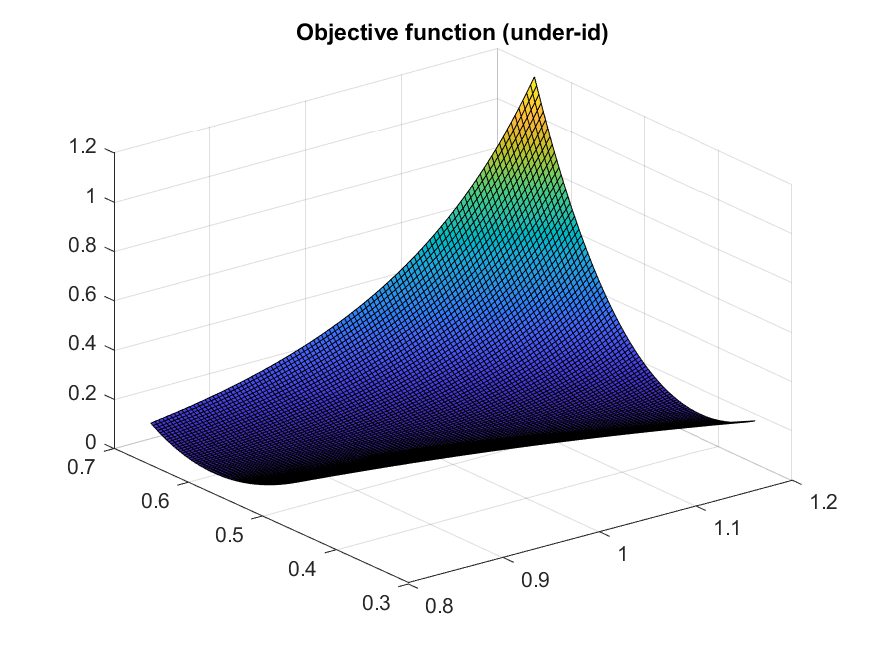
\includegraphics{obj_un}

Note that this objective function doesn't achieve zero, and also the shape is strange - it kind of has a trench moving diagonally across the $\rho \times \sigma$ space. This means that we cannot achieve identification, which is obvious. Here are the other objects that we are asked to report:

\begin{center}
\begin{tabular}{llll}
\hline 
  & b1 & b2 & SE \\ 
\hline 
rho & -0.989 & -1 & 326 \\ 
sigma & 0.184 & -0.106 & 8.57e+03 \\ 
\hline 
\end{tabular}

\begin{tabular}{cc}
\hline
\multicolumn{2}{c}{Jacobian} \\
\hline
-0.341 & -0.013 \\ 
-225 & -8.55 \\ 

\hline
\end{tabular}
\end{center}

Note that the "standard errors" here are massive because we don't have 'real' identification. The Jacobian is nearly collinear in its columns, so the only reason we can invert $\Delta g ' \hat{S}^{-1} \Delta g$ is because of numerical precision issues making the Jacobian slightly not exactly collinear. Our J-test (which should be exactly 0) is 47.5! Needless to say, the underidentified estimation doesn't work.

\subsection{Exactly-identified}

We now present the exactly-identified model. Results are substantially improved.

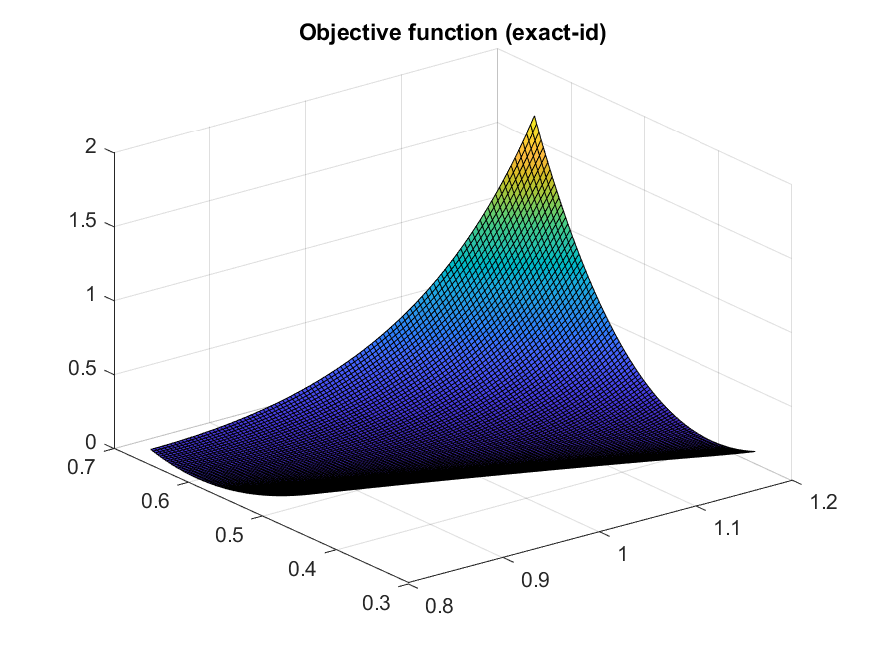
\includegraphics{obj_ex}

\begin{center}
\begin{tabular}{llll}
\hline 
  & b1 & b2 & SE \\ 
\hline 
rho & 0.543 & 0.543 & 0.0612 \\ 
sigma & 0.984 & 0.984 & 0.0552 \\ 
\hline 
\end{tabular}

\begin{tabular}{cc}
\hline
\multicolumn{2}{c}{Jacobian} \\
\hline
1.84 & 2.69 \\ 
2.27 & 1.39 \\ 

\hline
\end{tabular}
\end{center}

Note that our estimated parameters look identical but they are different in the first non-reported digit. Note also that we now no longer have collinear columns of the Jacobian. Our standard errors are much better now, unsurprisingly. Our J-test value is $2.77 \times 10^{-7}$ which is on an order smaller than the convergence parameters of the numerical minimizer in Matlab. So, numerically insignificant from zero.

\subsection{Over-identified}

We now present the overidentified model. Results are different than in the exactly-identified case, but not substantially different and not substantially better or worse. Our J-test in this case has a value 1.12, which while nonzero has a p value of 0.71 so we do not come remotely close to rejecting the null hypothesis, that the model is valid.

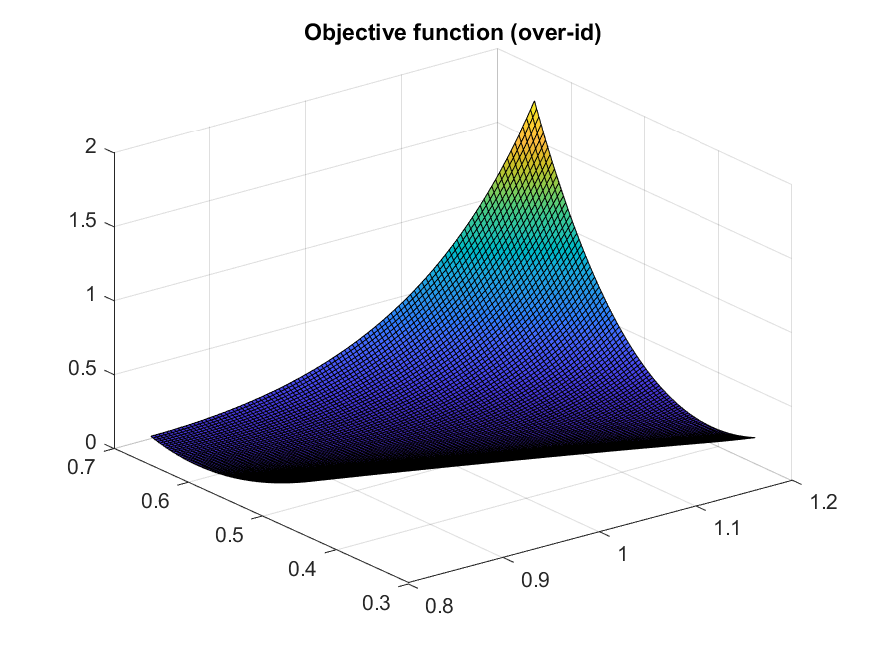
\includegraphics{obj_ov}

\begin{center}
\begin{tabular}{llll}
\hline 
  & b1 & b2 & SE \\ 
\hline 
rho & 0.484 & 0.477 & 0.063 \\ 
sigma & 0.97 & 0.965 & 0.0586 \\ 
\hline 
\end{tabular}

\begin{tabular}{cc}
\hline
\multicolumn{2}{c}{Jacobian} \\
\hline
0.105 & 0.0614 \\ 
1.6 & 2.62 \\ 
2.04 & 1.28 \\ 

\hline
\end{tabular}
\end{center}

In this version, we bootstrap the procedure. Histogram is below. Our histograms show that the distribution of bootstrapped estimates are approximately centered at the truth. Displayed are 50-bin histograms.

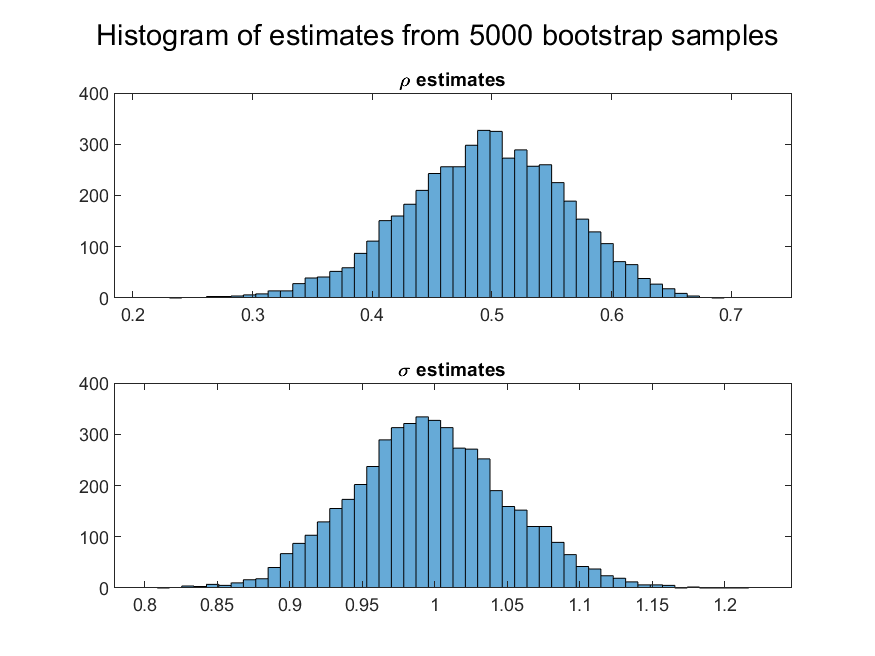
\includegraphics{boot}
% include table here with b1, b2, jacobian, standard errors.
\end{document}
